\section{Torsors and principal bundles}
\label{sec:torsors}

\subsection{Torsors}
\label{subsec:torsors}
We will review some definitions and facts, drawing on the excellent resource \cite{buchholtz2023central}.

\begin{mydef}
Let \( G \) be a group with identity element \( e \) (with the usual classical structure and properties). A \defemph{\( G \)-set} is a set \( X \) equipped with a homomorphism \( \phi:(G,e)\to\Aut(X) \). If in addition we have a term of type
\[ 
\mathsf{is\underscore torsor}(X,\phi)\defeq ||X||_{-1}\times \pit{x:X}\mathsf{is\underscore equiv}(\phi(-,x):(G,e)\to (X,x))
\] then we say \( (X,\phi) \) is a \defemph{\( G \)-torsor}. Denote the type of \( G \)-torsors by \( BG \). Denote the \( G \)-torsor given by \( G \) itself under right-multiplication by \( \reg{G} \).
\end{mydef}

A \( G \)-equivariant map from \( (X,\phi) \) to \( (Y,\psi) \) is a function \( f:X\to Y \) such that \( f(\phi(g,x))=\psi(g,f(x)) \). Denote the type of \( G \)-equivariant maps by \( X\to_G Y \).

\begin{mylemma}
(\cite{buchholtz2023central} Lemma 5.2). If \( (X,\phi),(Y,\psi):BG \) then there is a natural equivalence \( (X=_{BG}Y) \simeq (X\to_G Y) \).\qed
\end{mylemma}

\begin{mylemma}
(\cite{buchholtz2023central} Proposition 5.4). A \( G \)-set \( (X,\phi) \) is a \( G \)-torsor if and only if there merely exists a \( G \)-equivariant equivalence \( \reg{G}\to_G X \).\qed
\end{mylemma}

These lemmas lead to

\begin{mycor}
(\cite{buchholtz2023central} Corollary 5.5). The pointed type \( (BG,\reg{G}) \) is a \( \K(G,1) \), that is \( BG \) is connected and has a pointed equivalence \( \loopy BG\simeq_* G \).\qed
\end{mycor}

We call types \( X \) such that \( \loopy X\simeq_* G \) a \emph{delooping} of \( G \). So the type of \( G \)-torsors \( BG \) is a delooping of \( G \).

Suppose we have a basepoint \( b:BG \). Following \cite{buchholtz2023central} Section~4.3, another term \( X:BG \) is a torsor for the higher group \( \loopy_b(BG)\defeq (b=_{BG} b) \). In particular there is an action \( \alpha:(b=_{BG}b)\times X\to X \), and an equivalence \( (\alpha, \pr_2) : (b=_{BG}b)\times X\simto (X\times X)\).

If \( G \) is abelian then \( \K(G,1) \) can be delooped, and in fact can be delooped in a unique way, any number of times. In the next section we will learn how to proceed from a construction of \( \K(G, 1) \) to obtain \( \K(G, n) \).

\subsection{Bundles of Eilenberg-Mac Lane spaces}

To construct maps into \( \Kzt \) we will follow Scoccola\cite{sco}. When can a map into a connected component of the universe be factored through an Eilenberg-Mac Lane space?

\begin{mydef}
Let \( G \) be a group. Let \[ \EM(G,n)\defeq \BAut(\K(G,n))\defeq \sit{Y:\uni}||Y\simeq \K(G,n)||_{-1}\] be the connected component of \( \uni \) containing \( \K(G,n) \). A \defemph{\( \K(G,n) \)-bundle} on a type \( M \) is a map \( M\to\EM(G,n) \).
\end{mydef}

Scoccola constructs a map by composing 
\begin{itemize}
\item suspension \( \susp:\EM(G,n)\to\EM_{\bullet\bullet}(G,n) \) (see \cite{hottbook} §6.5), which maps into types with two points (denoted by the bullets),
\item \( (n+1) \)-truncation (see \cite{hottbook} §7.3),
\item forgetting a point \( F_\bullet:\EM_{\bullet\bullet}(G,n)\to \EM_{\bullet}(G,n) \),
\end{itemize}
to form the composition
\[ 
\EM(G,n)\xrightarrow[]{||\susp||_{n+1}} \EM_{\bullet\bullet}(G,n+1)\xrightarrow[]{F_\bullet}\EMp(G,n+1)
\]
to types with two points (north and south), then to pointed types (by forgetting the south point).

\begin{mydef}
Given \( f:M\to\EM(G,n) \), the \defemph{associated action of \( M \) on \( G \)}, denoted by \( f_\bullet \) is defined to be \( f_\bullet=F_\bullet\circ||\susp||_{n+1}\circ f \).
\end{mydef}

\begin{mythm}
\label{thm:sco}
(Scoccola\cite{sco} Proposition 2.39). A \( \K(G,n) \) bundle \( f:M\to\EM(G,n) \) factors through a map \( M\to\K(G,n+1) \), and so is a principal fibration, if and only if the associated action \( f_\bullet \) is merely homotopic to a constant map.
\end{mythm}

The above theory of classifying spaces should be relevant to any future project to bring the study of gauge theory into homotopy type theory. In this note we will be focused on the special case \( G=\zz \) and \( \EMzo \) and \( \Kzt \).

\begin{mynote}
Iterating the loop map gives the isomorphism \( \loopy^{(n+1)}:\EMp(G,n+1)\simeq \K(\Aut G,1) \) (see \cite{sco} Lemma 2.7). Theorem~\ref{thm:sco} therefore says that the map \( f \) factors through \( \K(G,n+1) \) if and only if the map into \( \K(\Aut G,1) \) is homotopic to a constant. In the case of \( G=\zz \), the map \( f_\bullet:M\to \K(\Aut \zz, 1) \) deserves to be called the first Stiefel-Whitney class of \( f \) and one can interpret its triviality as \emph{orientability}. . This point of view is discussed in Schreiber\cite{dcct} (starting with Example 1.2.138) and in Myers\cite{myersgood}.
\end{mynote}

\subsection{Pathovers}
\label{sec:pathovers}
Here we will recall basic facts from homotopy type theory. See for example \cite{hottbook} or \cite{egbert}. Suppose we have \( T:M\to\uni \) and \( P\defeq\sit{x:M}Tx \). Recall that if \( p:a=_M b \) then \( T \) acts on \( p \) with what's called the \emph{action on paths}, denoted \( \ap(T)(p):Ta=Tb \) (\cite{hottbook} §2.2). This is a path in the codomain \( \uni \) of \( T \). Type theory also provides a function called \emph{transport}, denoted \( \tr(p):Ta\to Tb \) (\cite{hottbook} §2.3) which acts on the fibers of \( P \). \( \tr(p) \) is a function, acting on the terms of the types \( Ta \) and \( Tb \), and univalence tells us this is the isomorphism corresponding to \( \ap(T)(p) \).

Type theory also tells us that paths in \( P \) are given by pairs of paths: a path \( p:a=_M b \) in the base, and a pathover \( \pi:\tr(p)(\alpha)=_{Tb}\beta \) between \( \alpha:Ta \) and \( \beta:Tb \) in the fibers (\cite{hottbook} §2.7). We can't directly compare \( \alpha \) and \( \beta \) since they are of different types, so we apply transport to one of them. We say \( \pi \) lies over \( p \). See Figure~\ref{fig:pathovers}.

\begin{figure}[H]
\centering
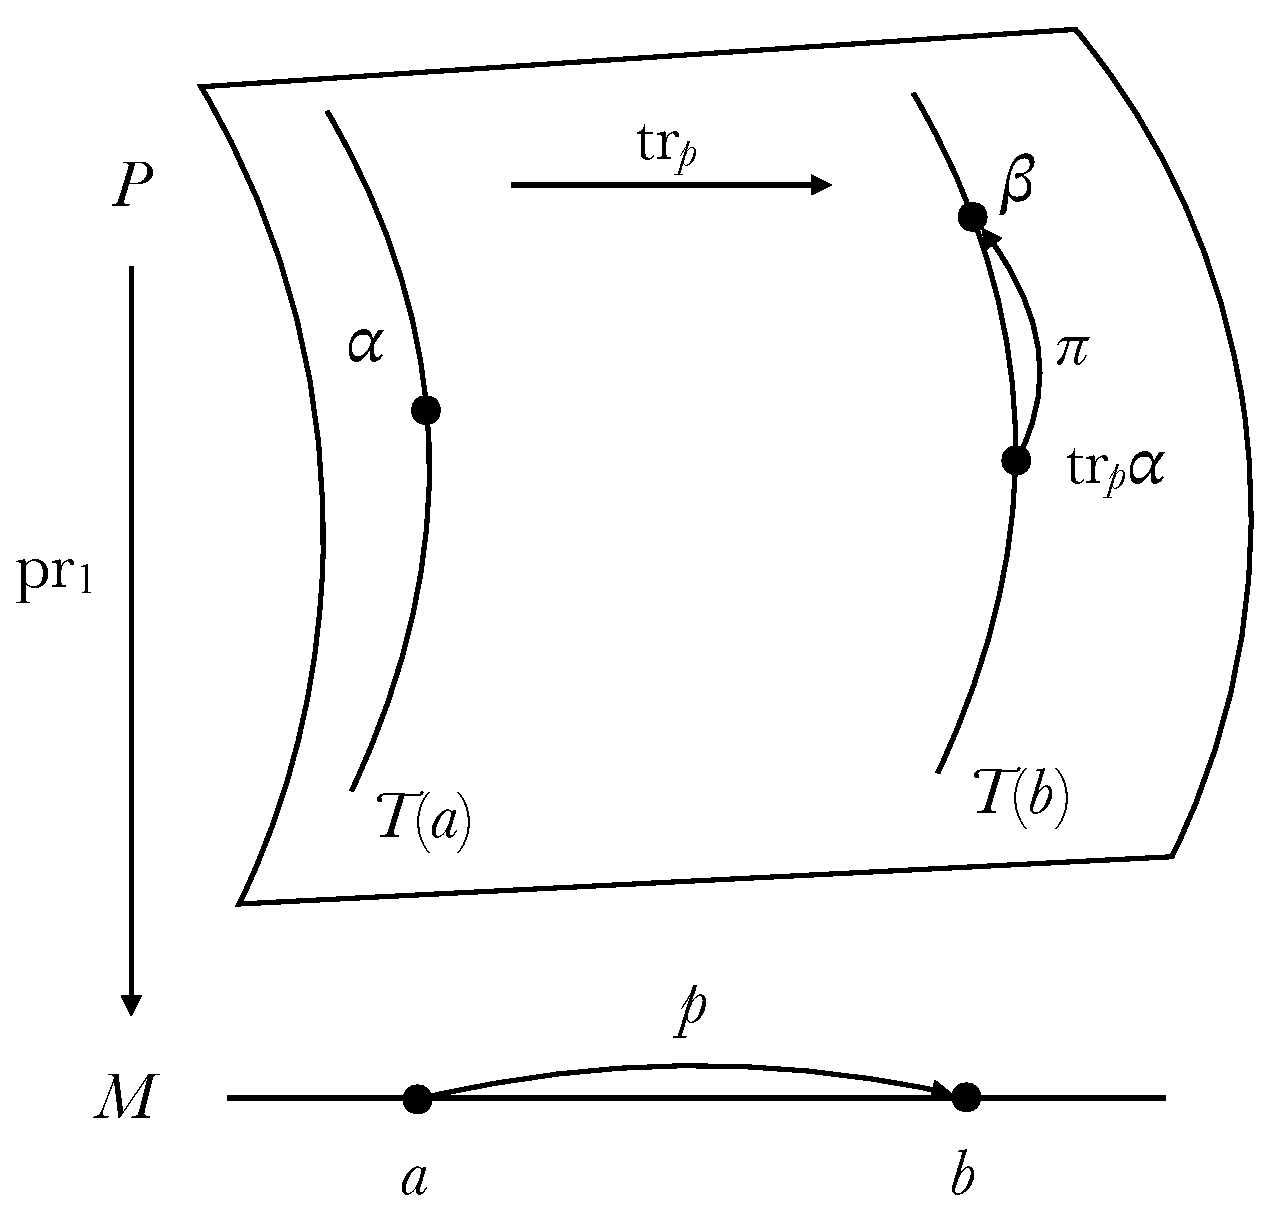
\includegraphics[width=200pt]{figs/pathovers.pdf}
\caption{A path \( \pi \) over the path \( p \) in the base involves the transport function.}
\label{fig:pathovers}
\end{figure}

Given functions \( \phi,\psi:A\to B \) between two arbitrary types we can form a type family of paths \( \alpha:A\to\uni \) by \( \alpha(a)\defeq(\phi(a)=_B\psi(a)) \). Transport in this family is given by concatenation as follows (see Figure~\ref{fig:transport_family_of_paths}), where \( p:a=_A a' \) and \( q:\phi(a)=\psi(a) \) (\cite{hottbook} Theorem 2.11.3):
\[ 
\tr(p)(q) = \phi(p)^{-1}\cdot q\cdot \psi(p)
\]
which gives a path in \( \phi(a')=\psi(a') \) by connecting dots between the terms \( \phi(a'), \phi(a), \psi(a), \psi(a') \). This relates a would-be homotopy \( \phi\sim\psi \) specified at a single point, to a point at the end of a path. We will use this to help construct such homotopies.
\begin{figure}[h]
\centering
\begin{tikzpicture}[
node distance = 20mm and 20mm,
V/.style = {circle, fill, draw=black, inner sep=1pt},
every edge quotes/.style = {auto},
arrow/.style={->,semithick}
]
\begin{scope}[nodes=V]
  \node[label=above left:\( \phi(a) \)] (1) {};
  \node[label=above right:\( \phi(a') \)] (2) [right=of 1]  {};
  \node[label=below right:\( \psi(a') \)] (3) [below=of 2]  {};
  \node[label=below left:\( \psi(a) \)] (4) [below=of 1]  {};
  \node[label=below:\( a \)] (5) [below=of 4]  {};
  \node[label=below:\( a' \)] (6) [below=of 3]  {};
\end{scope}
\draw[arrow]
        (2)  edge[swap, "\( \phi(p)^{-1} \)"] (1)
        (4)  edge["\( \psi(p) \)"] (3)
        (1)  edge[swap, "\( q \)"] (4)
        (5)  edge["\( p \)"] (6);
\end{tikzpicture}
\caption{Transport along \( p \) in the fibers of a family of paths. The fiber over \( a \) is \( \phi(a)=\psi(a) \) where \( \phi,\psi:A\to B \).}
\label{fig:transport_family_of_paths}
\end{figure}

Finally, recall that in the presence of a section \( X:M\to P \) there is a dependent generalization of \( \ap \) called \( \apd \): \( \apd(X)(p):\tr(p)(X(a))=X(b) \) which is a pathover between the two values of the section over the basepoints of the path \( p \) (\cite{hottbook} Lemma 2.3.4).
